\section{Cleaning for emittance scans}
\label{sec:emittance}

During 2015 data-taking, the LHC sometimes performed short van der Meer scans during collisions to track the beam emittance. This led to rapidly changing instantaneous luminosity across only a few lumi blocks, as shown in Figure~\ref{fig:emittance-scans}. These lumi blocks are marked with tolerable DQ defects because the reported luminosity is unreliable.

\begin{figure}
  \begin{center}
    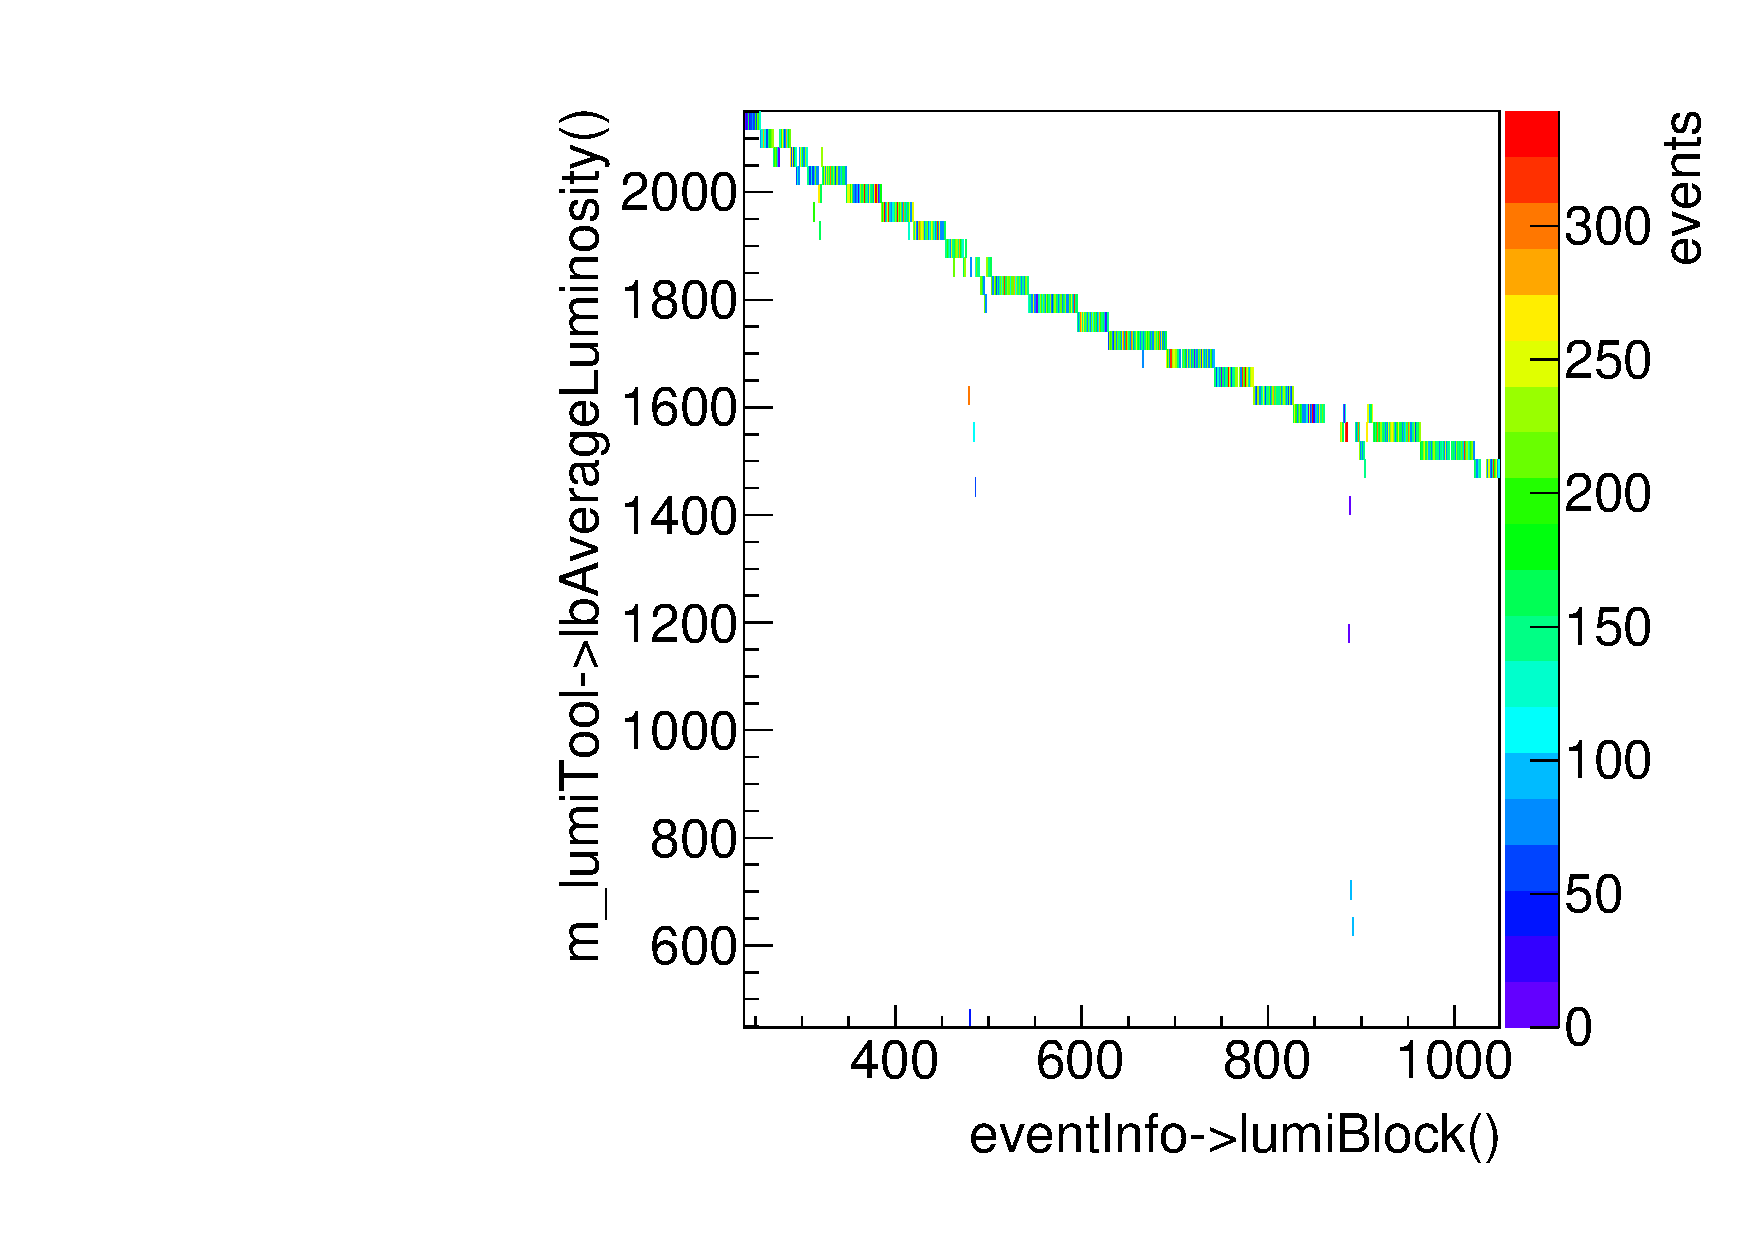
\includegraphics[width=0.45\textwidth]{./figures/lumi_vs_lb_00279685.pdf}
    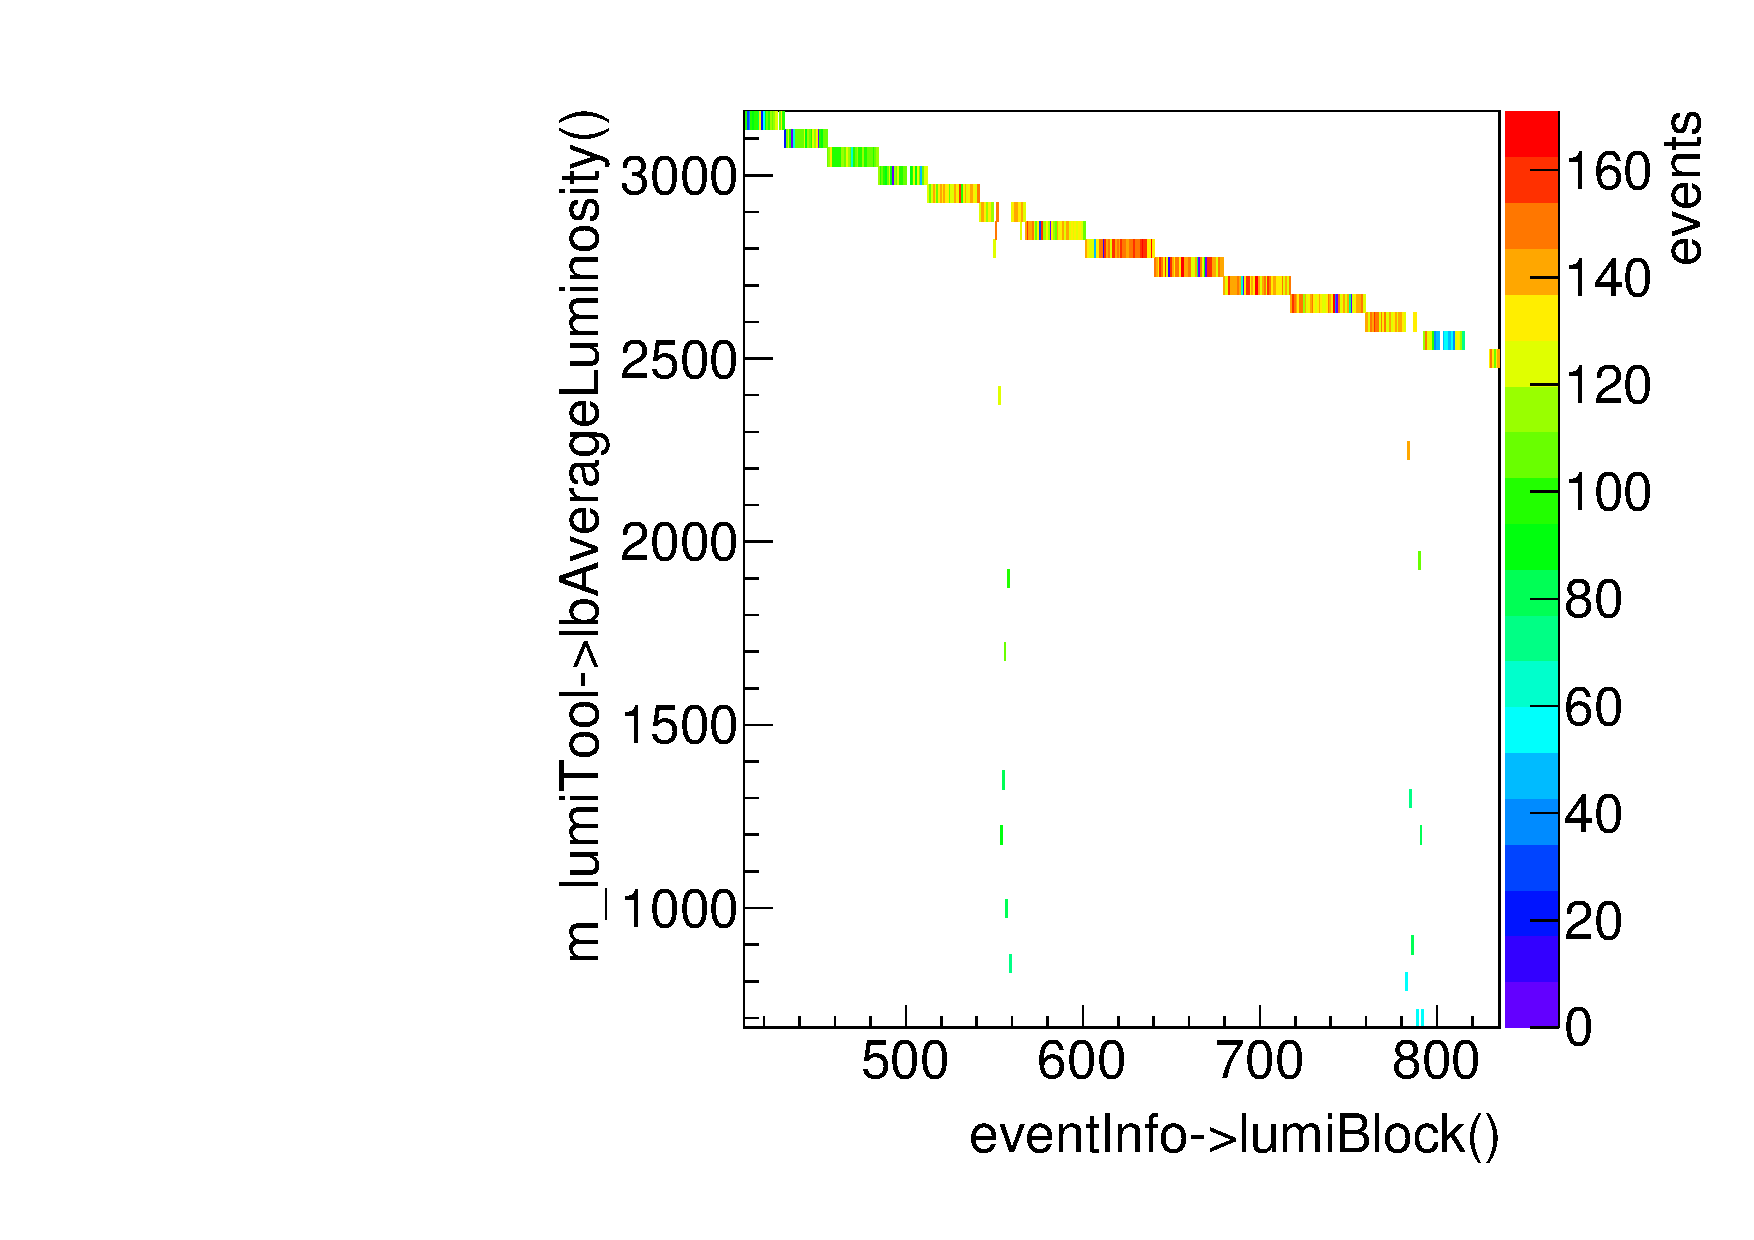
\includegraphics[width=0.45\textwidth]{./figures/lumi_vs_lb_00280464.pdf}
    \caption{Number of events in a given lumiblock and for a given instantaneous luminosity in Run 279685 (left) and 280464 (right). }
    \label{fig:emittance-scans}
  \end{center}
\end{figure}

The study of hit rates in the MDTs and CSCs depends heavily on the reported luminosity. Lumi blocks where the instantaneous luminosity is rapidly changing are therefore excluded from this study, as discussed in consultation with the \href{http://cern.ch/go/t7ND}{ATLAS Luminosity Group}.

